\chapter{Introduction}
\label{chap:intro}

In recent years computer hardware became increasingly powerful, allowing now even real time raytracing with the introduction of the RTX technology by NVIDIA in 2018 \cite{turing_whitepaper}.
In parallel to the advances in computer hardware the scenes to be rendered also became more and more complex reaching more than 70 GB of geometry data in a single shot in the film Coco \cite{pixarxpu}.
Besides the scene geometry, Textures in feature films can additonally consume up to a terabyte of memory \cite{arnold}.
While high detailed geometry and textures are required for close-up shots they impair performance when rendering them at large distances like in a landscape scene.
This is because rays have to be intersected with all triangles in an AABB regardless of the distance to the camera.
Additionally having high detailed geometry and textures at distance is prone to aliasing due to undersampling \cite{pbr}.
Tracing more rays per pixel combats this problem but is usually not feasible, since it increases the render time and has to be done every frame.
Alternatively we can use meshes with fewer triangles and textures that have less details.
Since the aliasing effect increases with distance we generate multiple \textit{levels of detail} (\acsp{lod}) and render them at a corresponding distance.
In this thesis we want to explore another approach for \acl{lod} rendering which combines the information of surface meshes and textures into a single representation using volumes.

We introduce fundamental concepts to this thesis in Chapter \ref{chap:fundamentals} and explain our method in Chapter \ref{chap:method}.
In Chapter \ref{chap:results_and_discussion} we present our results and discuss them before we look at further improvements to our approach in Chapter \ref{chap:future_work} and summarize our findings in Chapter \ref{chap:summary}.
First however, we take a look at the research that has been published in our domain in the following section.

\section{Related Work}
\subsection{Representing Dense Materials by Volumes}
Representing surfaces by volumes is a long standing problem in computer graphics.
Generally the visual appearance of volumes is determined by the choice of a phase function and the density respectively the extinction \cite{pbr}.
Therefore research mainly focuses on further improving these functions and the extinction behavior.

% The first work that suggested the use of volumes beyond the rendering of dust or smoke
An early work by \citeauthor{kajiya_rendering_fur_with_textures} uses three dimensional textures of density values to render fur \cite{kajiya_rendering_fur_with_textures}.
The authors store the particle density, a coordinate frame as well as parameters for diffuse and specular reflection functions in each texel \cite{kajiya_rendering_fur_with_textures}.
The density is obtained from a particle system which models the flow of a hair using the particle's trajectory \cite{kajiya_rendering_fur_with_textures}.
% The diffuse lighting component is transformed from the traditional lambertian reflectance model by integrating over the half cylindrical shape of a hair that faces the light source \cite{kajiya_rendering_fur_with_textures}.
% For specular reflection the authors

In a paper by \citeauthor{meng_multi_scale_modeling_and_rendering_of_granular_materials} volumetric representations of grains are used for efficient path tracing \cite{meng_multi_scale_modeling_and_rendering_of_granular_materials}.
For modeling the light scattering in the volume the authors use a tabulated phase function measured from simulating the light scattering of a single grain using ray-tracing \cite{meng_multi_scale_modeling_and_rendering_of_granular_materials}.
The extinction coefficient is computed from the simulation results as well since the authors also track the mean free-flight distance between successive interactions with grain \cite{meng_multi_scale_modeling_and_rendering_of_granular_materials}.
The authors observe a speedup of 2.1-30$\times$ compared to the surface representation \cite{meng_multi_scale_modeling_and_rendering_of_granular_materials}.
This is because next event estimation is not possible for grain that does not lie on the surface \cite{meng_multi_scale_modeling_and_rendering_of_granular_materials}.

Many recent contributions use the microflake model introduced by \citeauthor{microflake}, which models a volume by two-sided, randomly oriented flakes and therefore allows anisotropic media\cite{microflake}.
\citeauthor{zhao_building_volumetric_appearance_models} use this model to render fabric \cite{zhao_building_volumetric_appearance_models}.
The authors work with real fabric and scan it using computer tomography to obtain the density values for each voxel \cite{zhao_building_volumetric_appearance_models}.
To compute the orientation of the microflakes in each voxel, the authors fit cylinders to the scanned density field \cite{zhao_building_volumetric_appearance_models}.
For estimating the color and reflection properties the authors repeatedly render the volume and adjust the properties until the image matches a photograph of the fabric \cite{zhao_building_volumetric_appearance_models}.

\citeauthor{sggx} contributed another paper that uses the microflake framework \cite{sggx}.
The authors develop a new phase function which resembles the reflection properties of the GGX \ac{brdf} in volumes \cite{sggx}.
It can be used to substitute existing fiber-like scattering function as well as surface-like scattering functions \cite{sggx}.
This property makes it interesting for our thesis, since we want to represent surface meshes by volumes.
We therefore explain the theoretical background extensively in section \ref{subsec:phase_function}.

\subsection{Efficient Volume Rendering}
Although this thesis does not provide contributions to the optimization of volume rendering itself, using optimizations is key for competing with hardware accelerated ray tracing.
A popular algorithm in volume rendering is \textit{delta tracking} \cite{woodcock}, which needs a majorant of the particle density of the volume.
In its basic form this is a global majorant over the entire volume, however for strongly heterogeneous media it is more efficient to use local majorants \cite{novak_overview}.

In order to obtain local density majorants for delta tracking, \citeauthor{yue_space_partitioning} compare different space partitioning techniques regarding their performance implications \cite{yue_space_partitioning}.
These encompass a uniform grid partitioning, kd-trees and octrees \cite{yue_space_partitioning}.
The author evaluates their schemes on $8\times8\times8$ density grids and observe the highest speed-up compared to a global density majorant for the kd-tree with up to ${50\times}$ \cite{yue_space_partitioning}.
A drawback is the high construction time of more than $\SI{1.5}{\s}$ which is two orders of magnitudes slower than the octree and three orders of magnitues slower than the uniform partitioning \cite{yue_space_partitioning}.

\citeauthor{brick_grid} use local density majorants for their distance sampling and transmittance estimation \cite{brick_grid}.
Additionally their density majorant is available on different scales to account for high variation in the density \cite{brick_grid}.
The whole approach of \citeauthor{brick_grid} is optimized for the usage on a \ac{gpu}, which is why we use it in our research.
We go into further detail on this paper in section \ref{subsec:solving_beer_lambert_law_in_heterogeneous_media}.

% \subsection{Mesh voxelization}
\subsection{Level of Detail Approaches}
The theory for \ac{lod} rendering is motivated by the Nyquist-Shannon sampling theorem \cite{shannonsampling} which states that aliasing occurs when we sample a signal with less than twice the maximum frequency of the signal.
When keeping the sampling rate constant, we can therefore avoid aliasing by reducing the maximum frequency in the signal.

As mentioned in the introduction, the usual approach to achieve this goal for textures is to use increasingly blurry textures, which is generally called mipmapping \cite{mipmapping}.
This method generates new \acsp{lod} by recursively averaging the color of four neighboring texels until one texel remains on one or both sides of the texture \cite{mipmapping}.
Another approach for texture \acsp{lod} is the \ac{sat}.
For this method, a new texture is generated where each texel stores the sum of all texel values in the rectangle between the texel position and the lower left corner of the texture image \cite{crow_summed_area_tables}.
It is now possible to retrieve arbitrary filtered texture values by specifying upper and lower bounds of a rectangle for which the filtered color should be calculated \cite{crow_summed_area_tables}.
Subtracting the values at the upper left and lower right corner of this rectangle from the value at the top right and adding the value at the bottom left gives the summed intensity of the rectangle \cite{crow_summed_area_tables}.
Dividing by the area of the rectangle then gives the filtered color \cite{crow_summed_area_tables}.

For generating \acsp{lod} of surface meshes there are a number of strategies which we can classify in \textit{simplification}, \textit{subdivision}, \textit{tessellation} and \textit{voxel based} approaches.

% \noindent\textbf{Simplification}\linebreak
\subsubsection*{Simplification}
Mesh simplification techniques have in common that they remove geometry from an existing high detailed mesh while trying to preserve the visual appearcance \cite{realtime}.
This approach is followed in a paper by \citeauthor{hoppe_simplification} \cite{hoppe_simplification}.
They formulate the problem as the minimization of an energy function $E = E_{dist} + E_{rep} + E_{spring}$, where $E_{dist}$ measures the total squared distance of the mesh's points and $E_{rep}$ penalizes the number of vertices \cite{hoppe_simplification}.
$E_{spring}$ is a regularization term, which acts as if the edges between vertices were replaced by springs \cite{hoppe_simplification}.
Their algorithm randomly attempts to remove edges from the mesh and marks the change as preliminary if $E_{new} < E_{old}$ \cite{hoppe_simplification}.
In a second step one of the vertices in the neighborhood to this preliminary change is moved in order to minimize $E_{dist}$ and $E_{spring}$ while omitting self-intersections of the mesh \cite{hoppe_simplification}.

\citeauthor{peng_simplification} use edge collapse in a \ac{lod} context \cite{peng_simplification}.
They first apply a pre-processing step which determines the chronological order of the edge collapse \cite{peng_simplification}.
Based on this order, the vertices are restructured in memory, starting from vertices that exist in all \acp{lod} to vertices that only exist in detailed \acp{lod} \cite{peng_simplification}.
This allows to only load the vertices to the GPU that are required for the current \ac{lod} \cite{peng_simplification}.
The \ac{gpu} then applies the actual edge collapsing using one thread per triangle \cite{peng_simplification}.

% The authors of \citetitle{garland_heckbert_simplification} follow a similar approach, however they use a quadric error metric for the optimization procedure \cite{garland_heckbert_simplification}.
% \noindent\textbf{Subdivision}\linebreak
\subsubsection*{Subdivision}
Subdivision algorithms can also be seen as an instance of \ac{lod} approaches, since they start with a coarse mesh and iteratively produce smoother meshes.

\citeauthor{CATMULL1978350} introduced an algorithm that is now widely known as Catmull-Clark subdivision \cite{CATMULL1978350}.
The algorithm is not limited to triangle meshes but can be used with arbitrary polygons.
In the first step a new \textit{face point} is computed by calculating the average position of the vertices defining the face \cite{CATMULL1978350}.
Secondly, for every edge the authors compute the average position of the midpoint of this edge with the two adjacent points generated in step one, this gives new \textit{edge points} \cite{CATMULL1978350}.
Finally new \textit{vertex points} are generated by computing:
\begin{equation*}
	\frac{Q}{n} + \frac{2R}{n} + \frac{S(n-3)}{n},
\end{equation*}
$Q$ is the average of the $n$ new face points from step one that are adjacent to an old vertex point, $R$ is the average of the midpoints of all old edges that are incident on the old vertex points and $S$ is the old vertex point \cite{CATMULL1978350}.
% Figure \ref{fig:catmull_clark_new_points} illustrates the points that have been generated by these three steps.
Using these points new edges are added: Each new face point is connected to the adjacent new edge points from step two \cite{CATMULL1978350}.
Then the algorithm connects each new vertex point to the new edge points surrounding it \cite{CATMULL1978350}.
Figure \ref{fig:catmull_clark_subdivision} shows the subdivision of a cube after one iteration.
\begin{figure}[ht]
    \centering
    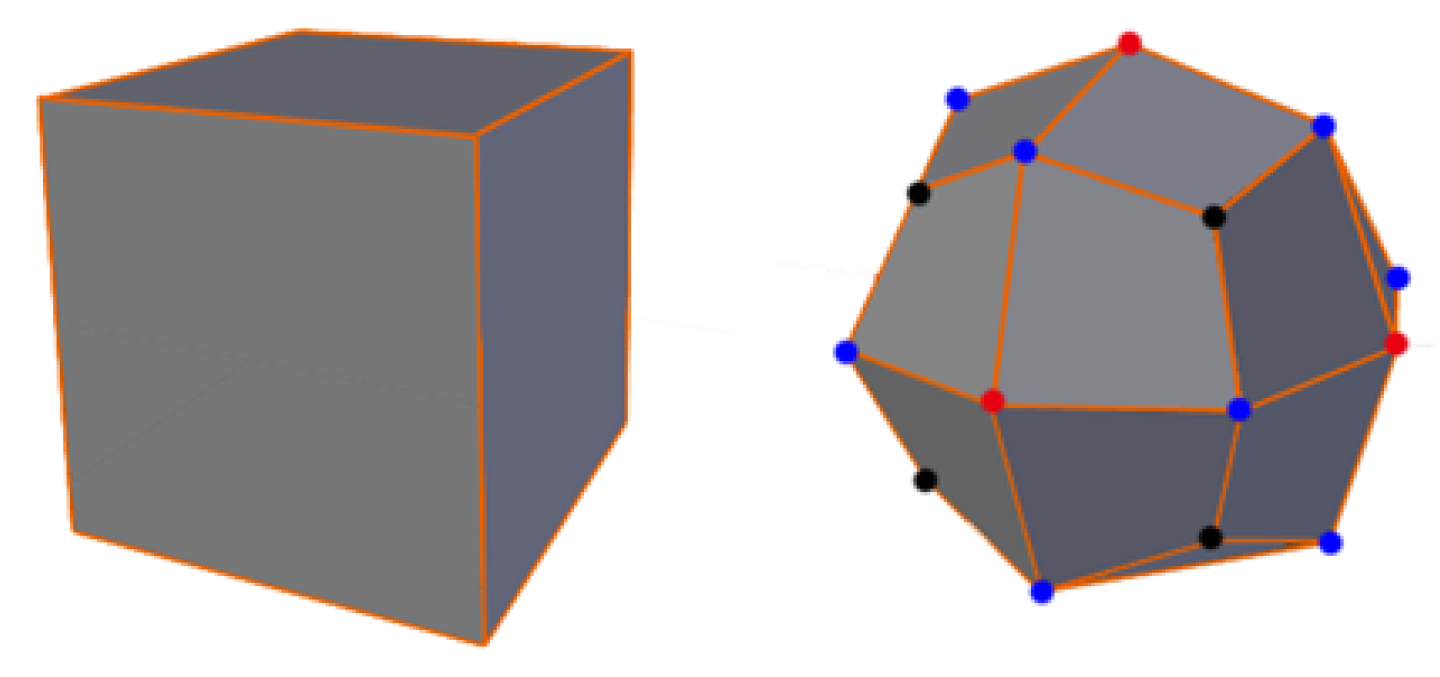
\includegraphics[width=0.5\linewidth]{img/catmull_clark_subdivision.png}
    % \caption[Points generated by the Catmull-Clark subdivision]{Points generated after the first three steps of the Catmull-Clark subdivision. Blue: Face points, generated in the first step. Pink: Edge points, generated in second step. Green: Vertex points, generated in third step. (Image from \cite{catmull_clark_step_3}).}
    \caption[First iteration of the Catmull-Clark subdivision]{First iteration of the Catmull-Clark subdivision on a cube mesh. The colors show in which step the point was generated. Red: Face points, generated in the first step. Blue: Edge points, generated in second step. Black: Vertex points, generated in third step (Image from \cite{cheng_catmull_clark_visualization}).}
    \label{fig:catmull_clark_subdivision}
\end{figure}

\citeauthor{loop_subdivision} later proposed another algorithm for triangle meshes \cite{loop_subdivision}.
In a first step, a new vertex is added at the midpoints of each edge \cite{loop_subdivision}.
Then the positions of existing and new vertices are updated using the weights in Figure \ref{fig:loop_subdivision}.
For existing points the new position is a weighted sum of all the surrounding vertices as well as the old position of the vertex \cite{loop_subdivision}.
New points take the immediate neighboring points into account as well as the other two points that form the adjacent triangles \cite{loop_subdivision}.
The weight $\beta$ is given by:
\begin{equation*}
    \beta = \frac{1}{n}(\frac{5}{8} - (\frac{3}{8} + \frac{1}{4}cos(\frac{2\pi}{n}))^2).
\end{equation*}
\begin{figure}[ht]
    \centering
    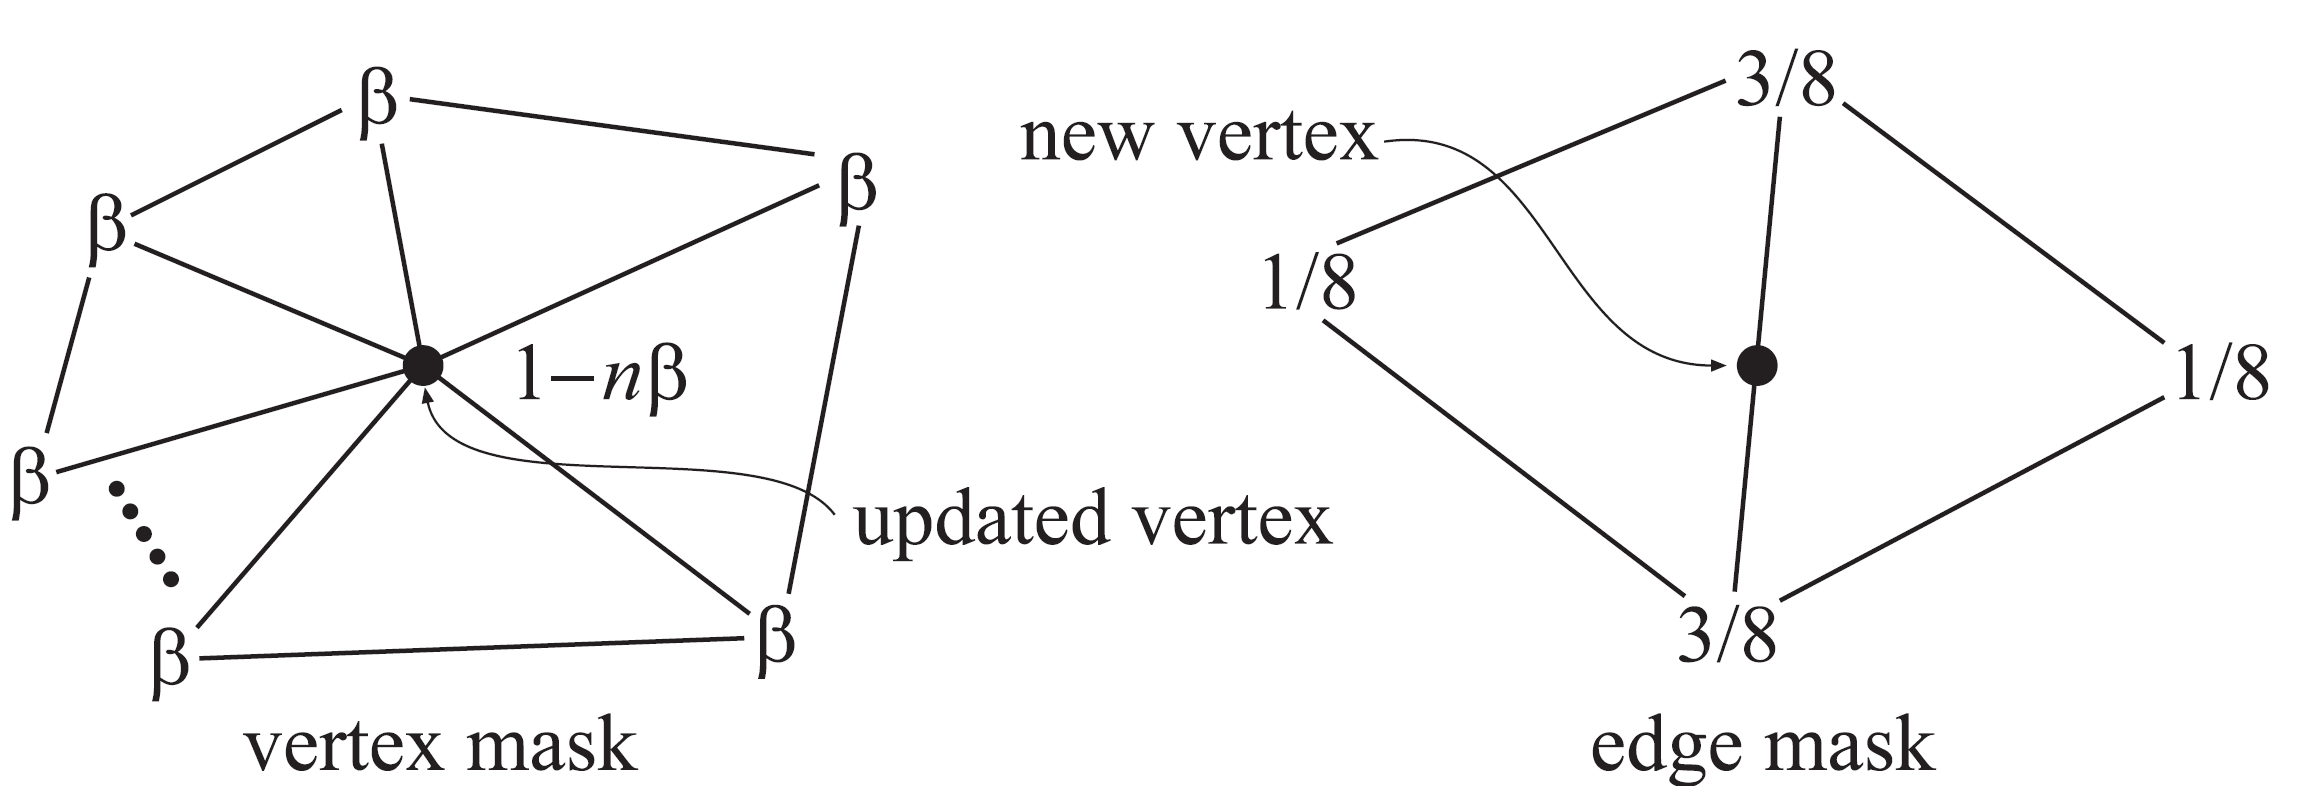
\includegraphics[width=0.5\linewidth]{img/loop_subdivision.png}
    \caption[Weights in Loop subdivision]{The weights for updating existing and new vertices. For existing points, the weight depends on the valence $n$ and a weight $\beta$, while new vertices are updated with constant values. (Image from \cite{realtime}).}
    \label{fig:loop_subdivision}
\end{figure}

\citeauthor{niessner_subdivision} explore how Catmull-Clark subdivision can be implemented on a \ac{gpu} \cite{niessner_subdivision}.
The authors use a table-driven approach where they first analyze the mesh on the \ac{cpu} and store the indices of the vertices that contribute to a subdivision in a table \cite{niessner_subdivision}.
Using this data they determine the new face, edge and vertex points with compute kernels on the \ac{gpu} by launching a thread for each new point \cite{niessner_subdivision}.
\citeauthor{niessner_subdivision} find that supporting this process with hardware tessellation for all regular faces improves the performance of their algorithm \cite{niessner_subdivision}.


\subsubsection*{Tessellation}
Tessellation is similar to subdivision as it also increases the number of triangles of a coarse mesh.
It typically refers to hardware tessellation which is a part of the rendering pipeline of modern \acp{gpu}.


An early work by \citeauthor{moreton_tessellation} compares the De Casteljau and the forward differencing algorithm for evaluating tensor product surfaces \cite{moreton_tessellation}.
These parametric surfaces are the basis for hardware tessellation.
The authors find that the De Casteljau algorithm produces more stable and precise results and supports evaluation at arbitrary parameter values.
Forward differencing uses only additions and has a complexity of $O(n)$ compared to a complexity of $O(n^2)$ for the De Casteljau algorithm.
This comes at the cost of being less precise and requiring a fixed parametric interval.
Since \citeauthor{moreton_tessellation} do not require the precision of De Casteljau they use forward differencing and propose a hardware implementation for the algorithm \cite{moreton_tessellation}.
The authors also present a way to produce continuous \acp{lod} by using fractional tessellation.
For that the tessellation is no longer uniform \cite{moreton_tessellation}.

An extensive overview of modern hardware tessellation is given in the paper \cite{niessner_tessellation} by \citeauthor{niessner_tessellation} \cite{niessner_tessellation}.
The authors show how tessellation integrates into current rendering pipelines as it is performed after the vertex shader and before the geometry shader \cite{niessner_tessellation}.
The first step is the hull shader which controls the tessellation rate of the parametric surface patch \cite{niessner_tessellation}.
For quads, four outer and two inner factors can be specified, while for triangles, three outer and one inner factor is available \cite{niessner_tessellation}.
Following the hull shader, the fixed function tessellator generates sample points and topology for a patch domain based on the tessellation factors \cite{niessner_tessellation}.
Finally the domain shader is executed for each sample location \cite{niessner_tessellation}.
It computes vertex attributes based on the tessellation factor, control points and domain sample locations \cite{niessner_tessellation}.
The authors also present various evaluation procedures for tensor product surfaces \cite{niessner_tessellation}.

\subsubsection*{Voxel Based}
Voxel based \ac{lod} approaches are special since they can not only encode the geometry of a model but also their texture.

\citeauthor{afra_voxel_lods} apply surface voxelization to large meshes with hundreds of millions of triangles \cite{afra_voxel_lods}.
The authors start by subdividing the geometry to build a kd-tree until each node in the tree contains no more than one triangle \cite{afra_voxel_lods}.
Starting from the root, voxelization is then performed on every third level for nodes with more than one triangle \cite{afra_voxel_lods}.
Their voxelization procedure is based on rasterization, where the triangles within a voxel are projected to all six sides of the voxel \cite{afra_voxel_lods}.
The authors then average normals and colors and store this average if the maximum absolute difference between the samples and the average is below a threshold \cite{afra_voxel_lods}.
If that is not the case, all six samples are stored \cite{afra_voxel_lods}.
\citeauthor{afra_voxel_lods} render the scene using ray tracing against the kd-tree \cite{afra_voxel_lods}.
The tree is traversed and for every voxel node, the screen space area of that node respectively the voxel is computed to determine whether to continue traversal \cite{afra_voxel_lods}.

Compared to \citeauthor{afra_voxel_lods}, \citeauthor{hybrid_mesh_volume_lods} propose a method for generating physically plausible density values for each voxel.
The authors use a hybrid approach between mesh and volume \acp{lod} \cite{hybrid_mesh_volume_lods}.
Their idea is to represent macroscopic surfaces (larger than the target resolution) as mesh \acsp{lod} while microscopic geometry (smaller than the target resolution) is represented by volumes \cite{hybrid_mesh_volume_lods}.
The first step in their pipeline is to seperate the macroscopic from the microscopic geometry \cite{hybrid_mesh_volume_lods}.
For a tree that would mean to seperate the trunk from the branches and leafs \cite{hybrid_mesh_volume_lods}.
The second step is to apply mesh simplification on the macroscopic surface while preserving the reflectance properties.
They achieve mesh simplification by using edge collapse, therefore they remove triangle edges which are smaller than the target resolution.
To preserve reflectance the authors update the diffuse and specular albedos of the remaining vertices by a weighted sum of the old vertices \cite{hybrid_mesh_volume_lods}.
The last step in their pipeline is the voxelization of the sub-resolution geometry.
The authors choose a ray casting approach to estimate the density for each voxel \cite{hybrid_mesh_volume_lods}.
This provides artifact-free voxelization and is therefore interesting for our research.
We go into the details of their filtering procedure in Section \ref{sec:transforming_meshes_into_volumes}.





\section{Contributions}
Our work provides the following contributions:
\begin{itemize}
    \item Implementation of a \ac{gpu} accelerated application for transforming triangle meshes into preferably equivalent volumetric representations in different resolutions and storing these representations in a common format.
    \item Extending these volumetric representations by attributes like color, normals and other material properties to closer approximate surfaces.
    \item Implementation of a \ac{gpu} based renderer capable of rendering surface meshes and volumes.
    \item A qualified heuristic to determine which \ac{lod} should be rendered.
    \item Evaluation of the image quality and rendering performance when triangle meshes are approximated by volumetric \acsp{lod}.
\end{itemize}
